%----------------------------------------------------------------------------
\section{Adatbázisrendszerek}
{\footnotesize Relációs, ER és objektumorientált modellek jellemzése. Adatbázisrendszer. Funkcionális függés. Relációalgebra és relációkalkulus. Az SQL.}
%----------------------------------------------------------------------------
\subsection{Relációs, ER és objektumorientált modellek jellemzése.}
\subsubsection{Bachmann-féle fogalomrendszer}
\begin{tabular}{|c|c|c|}
	\hline 
	& Absztrakt & Konkrét \\ 
	\hline 
	Egyed & Egyedtípus & Egyed-előfordulás \\ 
	\hline 
	Tulajdonság & Tulajdonságtípus & Tulajdonság-előfordulás \\ 
	\hline 
	Kapcsolat & Kapcsolattípus & Kapcsolat-előfordulás \\ 
	\hline 
\end{tabular}

\begin{description}[nosep]
	\item[Egyed] A valós világnak az az eleme (tárgy, jelenség, elképzelés, személy, fogalom stb.), amely a modellezés tárgyát képezi.
	\item[Egyedtípus] Az azonos tulajdonságtípusokkal rendelkező egyedek absztrakciója.
	\item[Tulajdonság] Az egyednek a modellezés szempontjából lényeges jellemzője.
	\item[Tulajdonságtípus] Az azonos szerepű tulajdonságok absztrakciója. A tulajdonságtípusok (attribútumok) osztályozása:
	\begin{enumerate}
		\item a tulajdonság-előfordulás szerkezete (összetettsége) szerint
		\begin{itemize}
			\item egyszerű (atom)
			\item összetett
		\end{itemize}
		\item a tulajdonság-előfordulás hány értéket vehet föl egyszerre
		\begin{itemize}
			\item egyértékű
			\item halmazértékű (többértékű)
		\end{itemize}
		\item a tulajdonság-előfordulás minden esetben megjelenik-e a háttértárolón (a fizikai adatbázisban)
		\begin{itemize}
			\item tárolt
			\item származtatot
		\end{itemize}
	\end{enumerate}
	\item[kapcsolat] A két vagy több egyedtípus egyedei között fennálló viszony.
	\item[Kapcsolattípus] Két vagy több egyedtípus közötti jól meghatározott viszony. Osztályozása:
	\begin{enumerate}
		\item A kapcsolat \textbf{foka} meghatározza, hogy hány egyedtípus vesz részt a kapcsolatban, eszerint beszélhetünk bináris (másodfokú), ternáris (harmadfokú),\dots kapcsolatról;
		\item A (bináris) kapcsolat \textbf{számossága} megmondja, hogy legfeljebb hány kapcsolat-előfordulásban vehet részt egy egyed-előfordulás. 3 fajtája lehet: 1:1, 1:N, M:N;
		\item A (bináris) kapcsolat \textbf{szorossága} meghatározza, hogy a kapcsolatban részt vevő egyedtípusok minden egyedének részt kell-e vennie legalább egy kapcsolat-előfordulásban. Eszerint a kapcsolat lehet kötelező, félig kötelező illetve opcionális.
	\end{enumerate}
\end{description}

\subsubsection{Relációs modell}
A relációs modell a legelterjedtebb modell. Ez köszönhető egyrészt annak, hogy a
személyi számítógépek elterjedésekor a megjelenő adatbázis-kezelő rendszerek ezen a modellen alapultak, valamint jól formalizált matematikai háttérrel rendelkezik.\\
A \textbf{tartomány (domain)} atomi értékek halmaza. Rendelkezik névvel, típussal és formátummal Jele: \textbf{D}\\
Az \textbf{attribútum} kijelöli az adott tartomány szerepét valamely rendszer esetén. Jele: \textbf{A}\\
A \textbf{relációs séma} ekkor az $R(A_1, ..., A_n)$ módon formalizálható, ahol R a séma neve, míg A i -k attribútumok. A relációs séma \textbf{foka} az attribútumainak száma.

A reláció ekkor a következő formalizmussal értelmezett:
$$r = r(R),\quad \text{ahol}\; r \subset dom(A_1) \times \dots \times dom(A_n)$$
Másszóval:
$$ r = \{t_1,\dots,t_m\},\quad\text{ahol }t_i = \langle v_{i1},\dots,v_{in}\rangle \;(1 \leq i \leq m)$$
a fent említett $v_{ij}\;(1\leq i \leq n)$ érték vagy $dom(A_j)$ eleme vagy NULL érték.
A relációséma az \emph{egyedtípusnak} feleltethető meg. A reláció sorai\footnote{formális modellben érték n-eseknek hívjuk őket.}, azaz  \textbf{rekordjai} az \emph{egyed-előfordulások} vagy \emph{kapcsolat-előfordulások}. A reláció kétdimenziós táblázattal szemléltethető. A táblázat oszlopait az attribútumok címkézik, a sorokban pedig a rekordok helyezkednek el. Megjegyzendő, hogy logikai szinten a rekordoknak nincs sorrendjük, a fizikai megvalósítás során mégis szükséges valamilyen sorrend felállítása.
\paragraph{A relációs modell megszorításai}
Az adatmodell megszorításainak csoportosítása:
\begin{itemize}[nosep]
	\item Az adatmodellben benne rejlő megszorítások: \textbf{modellalapú} vagy implicit megszorítások.
	\item Az adatmodell sémáiban közvetlenül kifejezett megszorítások: \textbf{sémaalapú} vagy explicit megszorítások.
	\item Olyan megszorítások, amelyeket nem lehet közvetlenül az adatmodell sémáiban kifejezni, és ezért az alkalmazói programokkal kell kifejezni és érvényre juttatni őket: \textbf{alkalmazásalapú} vagy szemantikus megszorítások vagy üzleti szabályok.
\end{itemize}
Sémaalapú megszorítások:
\begin{description}[nosep]
	\item[Tartomány megszorítás] Minden rekord minden egyes $A$ attribútumhoz tartozó értéknek a $dom(A)$ tartományból kell származnia. Ezen felül a $dom(A)$ tartományok elemei \emph{atomi értékeknek} kell lenniük.
	\item[Kulcs megszorítás] a relációsémának mindig rendelkeznie kell elsődleges kulccsal. Ennek bővebb tárgyalása később.
	\item[Egyedintegritási megszorítás] Az elsődleges kulcs nem lehet NULL értékű.
	\item[Hivatkozási integritási megszorítás] Egy $R_1$ relációséma $FK$-val jelölt attribútumhalmaza külső (idegen) kulcsa $R_1$-nek, amely hivatkozik az $R_2$ relációsémára, ha eleget tesz a következő feltételeknek:
	\begin{itemize}
		\item Az $FK$-beli attribútumoknak és az $R_2$ $PK$-val jelölt elsődleges kulcsattribútumainak páronként azonos a tartománya; ekkor azt mondjuk, hogy az $FK$ attribútumok hivatkoznak az $R_2$ relációsémára.
		\item Bármely $r_1(R_1)$ aktuális állapotának egy $t_1$ rekordjában egy $FK$-beli érték vagy megjelenik egy $r_2(R_2)$ aktuális állapotának valamely $t_2$ rekordjában $PK$ értékeként, vagy az értéke NULL. Az előbbi esetben $t_1[FK] = t_2[PK]$, ekkor azt mondjuk, hogy a $t_1$ rekord hivatkozik a $t_2$ rekordra.
	\end{itemize}
	Ha e két feltétel teljesül, egy hivatkozási integritási megszorítás áll fenn $R_1$-ről $R_2$-re vonatkozóan.
\end{description}
\subparagraph{Szuperkulcs, kulcs és elsődleges kulcs} 
\textbf{Szuper kulcsnak} nevezzük az olyan attribútum halmazt, amelynél nincs két olyan rekord, ahol az attribútumok rendre megegyeznek. Szuper kulcs mindig van. (Ha más nincs, akkor a séma összes attribútumának halmaza)\\
A \textbf{kulcs} olyan halmaz, ami szuper kulcsot alkot, de bármely attribútumot elhagyva belőle már nem kapunk szuper kulcsot (minimális szuper kulcs).\\
Egy relációsémának egynél több kulcsa is lehet. Ilyen esetben a kulcsok mindegyikét \emph{kulcsjelöltnek} hívjuk. A kulcsjelöltek közül a modellező feladata, hogy válasszon egy \textbf{elsődleges kulcsot}. Ezen kulcs fog a rekordok azonosítására szolgálni.\\
Legyen $R_1$ és $R_2$ két reláció. Az $R_1$ reláció $F_k$-val jelölt attribútum halmazát \emph{külső kulcsnak} nevezzük, ha az $F_k$-hoz tartozó attribútumok tartományai megegyeznek a $R_2$ elsődleges kulcsának tartományaival, és ha teljesül, hogy valamely $R_1$-beli rekord esetén vagy megegyezik valamely $R_2$-beli rekord elsődleges kulcsával, vagy NULL. (A kapcsolatok realizálják a külső kulcsok.)

\subsubsection{ER modell}
\begin{itemize}[nosep]
	\item egyed - kapcsolat modell
	\item a leggazdagabb modell
	\item sématervező eszköz, objektum alapszó, magasszintű eszköz, az 1. szemantikus modell
	\item koncepciós szinten tervezünk és grafikusan is megjelenik a modell
\end{itemize}
\begin{note}
Nincsen ER alapú adatbázis kezelő, ami azt jeleni, hogy le kell képezzük relációs sémává az ER modellt.
\end{note}
A modell kezeli az egyszerű és összetett, az egyértékű és halmazértékű (többértékű), valamint a tárolt és származtatott tulajdonságtípusokat.
\begin{definition}[Egyedtípusok]
	Azokat az egyedtípusokat, amelyek nem rendelkeznek saját kulcsattribútumokkal, \textbf{gyenge egyedtípusoknak} nevezzük. Ezzel ellentétben azokat a (hagyományos) egyedtípusokat, 	amelyeknek van kulcsattribútumuk, \textbf{erős egyedtípusoknak} nevezzük.
\end{definition}
\begin{definition}
	A gyenge egyedtípusoknak \textbf{részleges kulcsuk} (\emph{diszkriminátoruk}) van, amely azon attribútumok halmaza, amelyek egyértelműen azonosítják azokat a gyenge egyedeket, amelyek ugyanazon tulajdonos egyed(ek)hez kapcsolódnak.
\end{definition}
\begin{figure}[h]
	\centering
	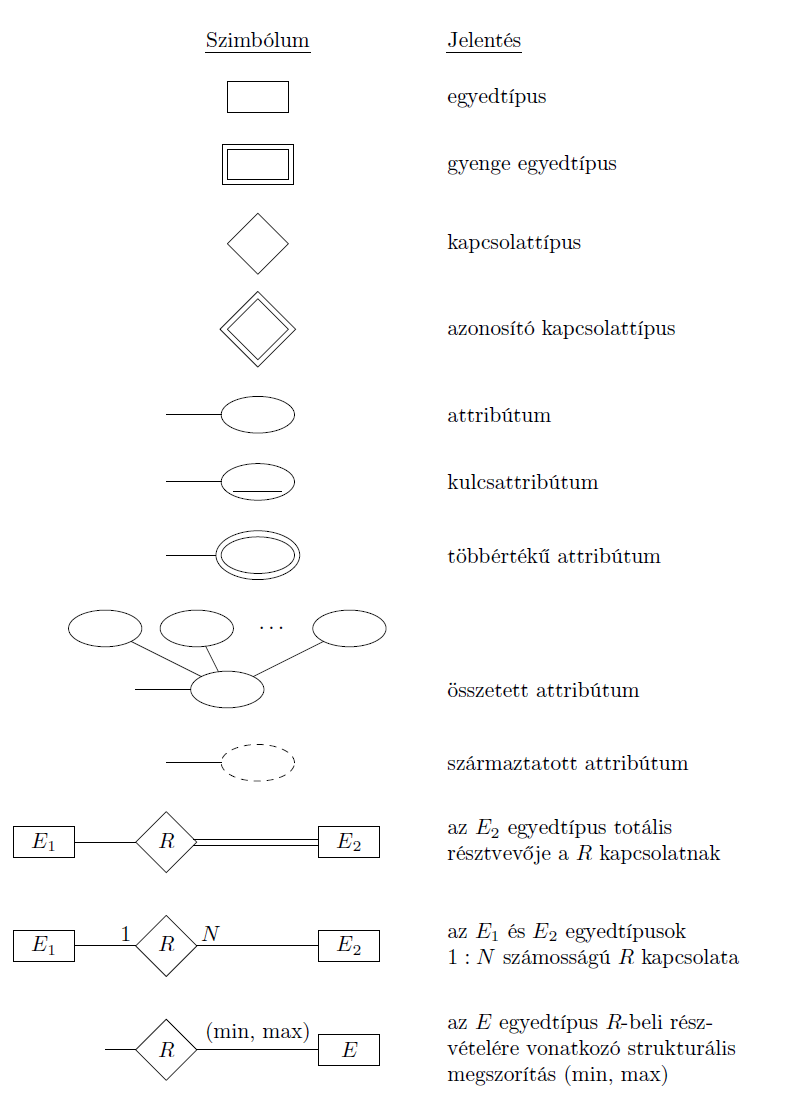
\includegraphics[width=0.7\linewidth]{fig/6-ER_symbols}
	\caption{ER model jelölései}
	\label{fig:6-ersymbols}
\end{figure}
Ennél a modellnél \emph{bármilyen fokszámú, számosságú és szorosságú kapcsolat} definiálható. Általában bináris kapcsolatokat használnak, mert ezeket a legkönnyebb leképezni más modellekre, de előfordulhat akár ötös fokszámú kapcsolat is. A kapcsolatok rendelkezhetnek attribútumokkal is. A számosságot az alapértelmezett 1:1, 1:N, M:N típusokon felül korlátozni lehet minimum és maximum határokkal minden egyedtípus felől. Például minimum kettő, maximum öt projektben vegyen részt egy dolgozó, és egy projektben minimum nyolc, maximum akármennyi dolgozó legyen.

A gyenge egyedtípusokhoz speciális azonosító kapcsolatra van szükség, ami jelzi, hogy valamelyik résztvevője gyenge. Emellett totális résztvevőnek hívjuk azt az egyedtípust, amelynek kötelező jelen lennie a kapcsolatban. A gyenge egyedtípusok ezért általában totális résztvevők.Egy kapcsolat lehet rekurzív is: minden résztvevő ugyanaz az egyedtípus. Ilyen például az, amikor az egyik dolgozó a más dolgozó felettese.
\begin{figure}[h]
	\begin{subfigure}{0.4\textwidth}
		\centering
		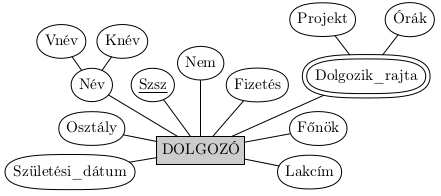
\includegraphics[width=\linewidth]{fig/6-ER_example1}
		\caption{}
		\label{fig:6-erexample1}
	\end{subfigure}
	\begin{subfigure}{0.6\textwidth}
		\centering
		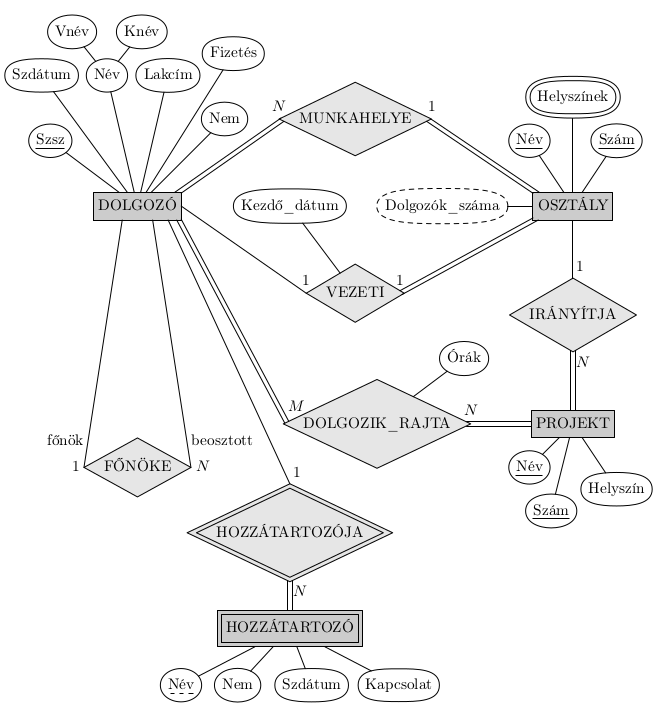
\includegraphics[width=\linewidth]{fig/6-ER_example2}
		\caption{}
		\label{fig:6-erexample2}
	\end{subfigure}
	\caption{ER séma példa}
	\end{figure}

\paragraph{ER séma leképezése relációs sémára}~\\
\begin{enumerate}[nosep]
	\item Erős egyedtípusok leképezése\\
	{\footnotesize Az ER séma minden E erős egyedtípusához rendeljünk hozzá egy R relációsémát, amely tartalmazza E összes egyszerű attribútumát. Az összetett attribútumoknak csak az egyszerű komponenseit adjuk hozzá R attribútumaihoz. Válasszuk E kulcs attribútumainak egyikét az R relációséma elsődleges kulcsául. Ha az E-ből választott kulcs összetett, akkor annak egyszerű attribútumai együttesen fogják alkotni R elsődleges kulcsát.}
	\item Gyenge egyedtípusok leképezése\\
	{\footnotesize Az ER séma minden W gyenge egyedtípusához rendeljünk hozzá egy R relációsémát, melynek attribútumai legyenek W összes egyszerű attribútuma és W összetett attribútumainak egyszerű komponensei. Továbbá adjuk hozzá R attribútumaihoz külső kulcs attribútumként azoknak a relációsémáknak az elsődleges kulcs attribútumait, amelyeket a domináns egyedtípusoknak feleltettünk meg; ezzel képezzük le a W -hez tartozó azonosító kapcsolattípust. R elsődleges kulcsa a tulajdonos egyedtípusok elsődleges kulcsainak és a W gyenge egyedtípus diszkriminátorának az együttese.}
	\item Bináris 1:1 számosságú kapcsolattípusok leképezése\\
	{\footnotesize Minden bináris 1:1 számosságú R kapcsolattípus esetén meg
		kell határozni az R-ben részt vevő egyedtípusokból képzett S és T relációkat. Három lehetséges megközelítés létezik: (1) külső kulcs használata, (2) összevonás és (3) keresztreferencia vagy kapcsoló reláció használata. Az első megközelítés a leghasznosabb, és azt célszerű alkalmazni, hacsak bizonyos feltételek nem állnak fenn, ahogy azt mindjárt látni fogjuk:}
	\begin{enumerate}
		\item külső kulcs használata\\
		{\footnotesize Válasszuk ki az egyik relációt (mondjuk S-t) és vegyük fel S külső kulcsaként T elsődleges kulcsát. Célszerű S-nek azt a relációt választani, amelyiket abból az egyedtípusból képeztünk le, amelyik totális résztvevője az R kapcsolatnak. Vegyük fel továbbá R egyszerű attribútumait, illetve R összetett attribútumainak egyszerű komponenseit S attribútumaiként. (Azt is megtehetnénk, hogy S (a totális résztvevő) elsődleges kulcsát vesszük fel T külső kulcsaként, de ebben az esetben T minden olyan rekordjánál, amelyik nem vesz részt a kapcsolatban, ehhez a külső kulcshoz null értéket kellene rendelni.)}
		\item összevonás\\
		{\footnotesize Egy másik lehetőség az 1:1 kapcsolatok leképezésére, ha a két egyedtípust és a kapcsolatot egyetlen relációba vonjuk össze. Ezt akkor tehetjük meg, ha mindkét egyedtípus totális résztvevője a kapcsolatnak.}
		\item kereszthivatkozás v. kapcsoló reláció használata\\
		{\footnotesize A harmadik lehetőség, hogy felveszünk egy harmadik R relációt abból a célból, hogy kereszthivatkozással lássuk el a két egyedtípusból képzett S és T relációk elsődleges kulcsait. Ahogy látni fogjuk, ezt a megközelítést alkalmazzuk a bináris M:N kapcsolatoknál is. Az R relációt kapcsoló relációnak nevezzük, mert R minden rekordja egy kapcsolat-előfordulást reprezentál, amely S egy rekordját T egy rekordjával kapcsolja össze.}
	\end{enumerate}
	\item Bináris 1:N számosságú kapcsolattípusok leképezése\\
	{\footnotesize Minden bináris 1:N számosságú R kapcsolattípus esetén meg kell határozni azt az S relációt, amelyiket a kapcsolattípus N-oldali egyedtípusából képeztünk. Vegyük fel S külső kulcsaként az R-ben részt vevő másik egyedtípusból képzett T reláció elsődleges kulcsát; mindezt azért tesszük, mert az N-oldali egyed-előfordulások a másik oldalról legfeljebb egy egyed-előforduláshoz tartoznak. Vegyük fel továbbá R egyszerű attribútumait, illetve R összetett attribútumainak egyszerű komponenseit S attribútumaiként.}
	\item Bináris M:N számosságú kapcsolattípusok leképezése\\
	{\footnotesize Minden bináris M : N számosságú R kapcsolattípus esetén hozzunk létre egy új S relációt, amely R-et reprezentálja. Vegyük fel S külső kulcsaként a kapcsolatban részt vevő egyedtípusokból képzett relációk elsődleges kulcsait; ezek együttese alkotja S elsődleges kulcsát. Vegyük fel továbbá R egyszerű attribútumait, illetve R összetett attribútumainak egyszerű komponenseit S attribútumaiként. Egy M:N kapcsolatot nem tudunk egyetlen külső kulccsal reprezentálni az egyik résztvevő relációban: létre kell hoznunk egy külön S kapcsoló relációt}
	\item Többértékű attribútumok leképezése\\
	{\footnotesize Minden egyes A többértékű attribútum esetén hozzunk létre egy új R relációt. Ez az R reláció tartalmazzon egy, az A-nak megfelelő attribútumot, valamint annak a relációnak a K elsődleges kulcsát – R külső kulcsaként –, amelyet az A-t tartalmazó egyedtípusból vagy kapcsolattípusból képeztünk. R elsődleges kulcsát A és K együttese alkotja. Ha a többértékű attribútum összetett, akkor az egyszerű komponenseit vegyük fel R attribútumaiként.}
	\item N-ed fokú kapcsolattípusok leképezése\\
	{\footnotesize Minden N-edfokú R kapcsolattípus esetén, ahol N > 2, hozzunk létre egy új S relációt, amely R-et reprezentálja. Vegyük fel S külső kulcsaként a kapcsolatban részt vevő egyedtípusokból képzett relációk elsődleges kulcsait. Vegyük fel továbbá R egyszerű attribútumait, illetve R összetett attribútumainak egyszerű komponenseit S attribútumaiként. S elsődleges kulcsa általában az összes külső kulcs együttese. Ha azonban az R-ben részt vevő valamely E egyedtípusból csak egy rekord vehet részt a kapcsolatban (számossági megszorítás), akkor S elsődleges kulcsának nem kell tartalmaznia az E-ből képzett E 0 relációra hivatkozó külső kulcsot.}
\end{enumerate}

\subsubsection{OO modell}
Az adatbázis tervezésben már elérhető az OO paradigma is. Az ODL egy példa az
objektumorientált definíciós nyelvekre. A tervezés során a valós világ egyedeit
objektumoknak tekintjük.
\paragraph{az objektum négy jellemzője}~\\
\begin{enumerate}[nosep]
	\item azonosító (OID)
	\item név (adható neki egyedi név egy adatbázison belül, ezzel hivatkozhatunk rá)
	\item élettartam (perzisztens vagy tranziens)
	\item struktúra -> milyen típus konstruktorok segítségével hoztuk létre az objektumot.
\end{enumerate}
Az azonos típusú attribútumokkal rendelkező fogalmak tartoznak egy osztályba. Az osztályok rendelkeznek attribútumokkal, metódusokkal és kapcsolatokkal. Az osztály definíciója:
\begin{verbatim}
interface osztálynév [:szuper típus]
( [key kulcsattribútumok] )
{
  attribútumok
  kapcsolatok
  metódusok
}
\end{verbatim}
Az attribútumaik lehetnek egyszerűek (atomiak), illetve különféle kollekció típusúak.(halmaz, lista, struktúra, tömb) Megadásuk: attribute típus név;

A kapcsolatoknak nincs attribútumuk, és nem lehet sokágú kapcsolatokat létrehozni. Ezek megvalósításához egy új, a kapcsolatot reprezentáló osztályt kell létrehozni. Definiálható viszont egy, és kétirányú kapcsolat is. Megadásuk: relationship típus név [inverse inverzkapcsolat];

A metódusok az objektumra alkalmazható műveleteket írják le. A modell ezeknek csak a szignatúráját kezeli, a megvalósításukat nem. Megadásuk: [típus] függvénynév(paraméterek); 

Az ODL-ben az elsődleges kulcs egy vagy több olyan attribútum, amelynél nincs két olyan objektum, melyre ezek mindegyike megegyezik. Egy attribútum: egyszerű; több attribútum: összetett kulcs.

Az OO paradigmának megfelelően az osztályok kiterjeszthetőek. Ekkor a szülő osztály minden attribútuma, kapcsolata és metódusa átkerül az alosztályba. Egy osztálynak több szülője is lehet.

ODMG szabvány /Object Data Managament Group/ objektumorientált adatbázisrendszerekkel
foglalkozó cégek tömörülése
1993: az első ilyen szabvány megjelenése
Több részből áll a szabvány és a modell is:
\begin{itemize}
	\item objektummodull leírása
	\item objektum definíciós nyelv (ODL)
	\item objektum lekérdező nyelv (OQL)
	\item kapcsolódások az OO programnyelvekhez / C++, Java, Smalltalk /
\end{itemize}


\subsection{Adatbázisrendszer.}
Az adatbázisrendszer számítógépekből, adatokból, kezelő szoftverből és kezelőkből áll. Az adatbázis a \textbf{meta-adatbázisból} és a \textbf{fizikai adatbázisból} tevődik össze. A meta-adatbázis az adatbázis szerkezetére vonatkozó információk összessége, a fizikai adatbázis pedig az egyed-előfordulások összessége. A kezelő rendszer valamilyen szoftver (\textbf{DBMS}), mindig konkrét operációs rendszer alatt fut, gyakran sok funkciót átvesz tőle. Programozhatóság szerint létezik \textbf{saját nyelvű} (része valamilyen programozási eszközrendszer, jellemzően eljárásorientált, imperatív jellegű) és \textbf{befogadó nyelvű} (utasításokkal rendelkezik lekérdezésekhez, manipulációhoz, programozáshoz magas szintű nyelven írt programot kell hozzáilleszteni). A korábbi rendszerek jellemzően befogadóak voltak. A saját nyelv általában kevesebbet tud, mint a magas szintű nyelvek.

A felhasználó tényleges adatokhoz csak a DBMS-en keresztül férhet, az operációs rendszert használva. A fizikai adatbázist kezelő utasítások összessége az \textbf{adatmanipulációs nyelv} (DML), míg a szerkezet (séma) leírására alkalmas nyelvrész az \textbf{adatleíró nyelv} (DDL). Mellettük létezik még az \textbf{adatvezérlő nyelv} (DCL), mely a jogosultságokkal, tranzakciókkal kapcsolatos utasításokat tartalmazza. A teljes adatbázisrendszer felügyeletéért felelős személyek az \textbf{adminisztrátorok} (DBA).

Az egyes felhasználói csoportok aszerint különíthetőek el, hogy hozzáférésük során mi jellemző munkájukra. Az \textbf{eseti felhasználók} eseti kérdéseket tesznek fel, optimális eszközrendszerük interaktív, kérdései véletlenszerűek és nagyon különböző információkra vonatkoznak. A \textbf{parametrikus felhasználók} szűk, előre meghatározott kérdéskörben tesznek fel kérdéseket, eszközrendszerük jól programozható, paraméterezhető alkalmazást futtatnak. A szakemberek ismerik a DBMS lehetőségeit, alkalmazásokat írnak és fejlesztenek tovább, nagy mennyiségű adattal dolgoznak.

Egy adatbázisrendszeren belül a legfontosabb erőforrás az adat.
\textbf{Cél:} a felhasználók optimális kiszolgálása az adatbázisrendszeren belül.

Az adatbázis architektúra \emph{fizikai (belső)}, \emph{logikai (külső)} és \emph{koncepcionális} szintekből áll. Fizikai szinten az adatok fizikai elhelyezkedését és az elérési módokat kell leírni. Koncepcionális szinten az adatbázissal, mint logikai egységgel kell foglalkozni, a sémát kell leképezni fizikai szintre (rekordtípusok, tulajdonságtípusok, hozzáférések megadása). Logikai szinten jelenik meg a felhasználói csoportokra történő felosztás, az alsémák megadják, hogy a egyes csoportok mit látnak az adatbázisból.

Az adatbázis-építés során először elemzés, tervezés, modellezés útján kell eljutni sémához és alsémákhoz koncepcionális szinten, majd e sémát leírva meta adatbázisba kerül (üres adatbázis), fel kell tölteni a fizikai adatbázist, végül lekérdezések útján nyerhetők ki a szükséges információk.

\subsection{Funkcionális függés.}
\begin{definition}[1]
	Legyen $R(A_1 , A_2 \dots A_n)$ relációséma és $X$, $Y$ az $\{A_1 , A_2 \dots A_n\}$ attr. halmaz részhalmazai. $X$-től funkcionálisan függ $Y$, ha bármely $R$ feletti $T$ tábla esetén valahányszor két sor megegyezik $X$-n, akkor megegyezik $Y$-n is. Jele: $X \to Y$
\end{definition}
\begin{definition}[2]
	Az $R$ két attribútumhalmaza, $X$ és $Y$ között, $X \to Y$-nal jelölt funkcionális függés előír egy megszorítást azokra a lehetséges rekordokra, amelyek egy $R$ fölötti $r$ relációt alkothatnak. A megszorítás az, hogy bármely két, $r$-beli $t_1$ és $t_2$ rekord esetén, amelyekre $t_1[X] = t_2[X]$ teljesül, teljesülnie kell $t_1[Y] = t_2[Y]$-nak is.
\end{definition}
\begin{note}
	Két attribútumhalmaz közötti összefüggést/kapcsolatot írja le. Legyen X és Y az R reláció két attribútumhalmaza! Y funkcionálisan függ X-től ( vagy X funkcionálisan meghatározza Y-t), ha bármelyik két rekord esetén abból, hogy a két rekord X attribútum-értékei megegyeznek következik, hogy az Y attribútum-értékei is megegyeznek.
\end{note}
\begin{note}
	A funkcionális függés nem két irányú kapcsolat!\\
	Ha $X \to Y$ és $Y \to X$ egyszerre áll fenn, akkor azt mondjuk, hogy $X$ és $Y$ \textbf{kölcsönös funkcionális függésben} áll egymással.
\end{note}

\begin{theorem}[A funkcionális függés tulajdonságai]~\\
	\begin{enumerate}[nosep]
		\item reflexivitás: $\text{Ha} X\subseteq Y,\quad \text{akkor} X \to Y$\\
			{\small\bfseries Egy attribútumhalmaz mindig meghatározza önmagát, vagy saját maga bármilyen részhalmazát.}
			{\footnotesize $X = \{A_1,A_2,A_3,A_4\}$\\
			$Y = \{A_2,A_3\}$\\
			$t_1[X] = t_2[X] \implies t_1[Y]=t_2[Y]$}
		\item augmentivitás: $\{X\to Y\}\quad \implies XZ \to YZ $\\
			{\small\bfseries egy funkcionális függés mindkét oldalának ugyanazzal az attribútumhalmazzal történő bővítése újabb érvényes funkcionális függést eredményez.}
			
		\item tranzitivitás: $\{X \to Y,Y \to Z\}\quad \implies X \to Z$\\
			{\small\bfseries a funkcionális függések tranzitívak.}
		\item dekompozíció: $\{X \to YZ\}\quad \implies X \to Y$\\
			{\small\bfseries egy funkcionális függés jobb oldaláról eltávolíthatunk attribútumokat.}
		\item additivitás szabályai: $\{X \to Y,X \to Z\}\quad \implies X \to YZ$\\
			{\small\bfseries funkcionális függések egy $\{X \to A_1 ,X \to A_2 ,\dots,X \to A_n \}$ halmazát összevonhatjuk egyetlen $X \to \{A_1 ,A_2 ,\dots,A_n \}$ funkcionális függéssé.}
		\item pszeudotranzitivitás: $\{X \to Y,WY \to Z\}\quad \implies WX \to Z$\\
	\end{enumerate}
\end{theorem}
\begin{definition}[Triviális függés]
	Egy $X \to Y$ funkcionális függés \textbf{triviális}, ha $X \subseteq Y$ (Y részhalmaza X-nek), egyébként nemtriviális.
\end{definition}
\begin{theorem}[Triviális függés]
	Egy $X \to Y$ funkcionális függés \textbf{teljesen nem triviális}, ha $X\cap Y=\emptyset$ ($X$ és $Y$ metszete üres halmaz).
\end{theorem}

\subsection{Relációalgebra és relációkalkulus. }
A relációalgebra egy absztrakt kezelő nyelv. Minden relációs algebrai művelet eredménye egy reláció lesz.

\subsubsection{Unáris műveletek}
\begin{description}[nosep]
	\item[Szelekció ($\sigma$)] Egy adott reláció rekordjainak egy részhalmazát adja, amely részhalmazba egy feltételt teljesítő rekordok fognak beletartozni. Ez a feltétel a szelekciós feltétel, ami általában egy logikai kifejezés. Ebben a kifejezésben hasonlító és logikai műveleti jelek lehetnek. Formálisan a műveletben attribútumok és konstansok vannak.\\
	$$\sigma_\text{feltétel}(\text{relációs\_séma\_név})$$
	Az eredményül kapott reláció fokszáma megegyezik a kiindulási reláció fokszámával. A kapott rekordok száma kisebb vagy egyenlő mint az induló rekordok száma.\\
	pl.: $\sigma\text{ feltétel}_{=4 \text{OR}\;\text{DNO}=5}(EMPLOYEE)$\\
	A szelekció kommutatív művelet: $\sigma_{f1}(\sigma_{f2}(R))=\sigma_{f2}(\sigma_{f1}(R))$\\
	Lényeges az a szemlélet a konkrét megvalósításnál, hogy szelekció a rekordokon egyenként hajtódik végre. Szelekciósorozat mindig értelmezhető egyetlen szelekcióként:
	$\sigma_{f1}(\sigma_{f2}\dots(\sigma_{fn}(R))\dots)=\sigma_{f1 \text{AND} f2 \text{AND} \dots fn}(R)$\\
	A szelekció logikai szinten : a táblázatból kiemelek bizonyos sorokat.\\
	SQL: \verb|SELECT * FROM R WHERE szelekciós feltétel|
	\item[Projekció ($\pi$)] A kiinduló relációból kiválaszt bizonyos attribútumokat, és az eredményrelációba csak ezen attribútumokhoz tartozó értékeket viszi át.
	$$\pi_\text{attribútum\_lista}(\text{reláció\_séma\_név})$$
	Logikai szint: a táblából oszlopok kiválasztása.\\
	pl.: $\pi_\text{FNAME,LNAME,BDATE}(\text{EMPLOYEE})$
	Az attribútumlistán az attribútumok sorrendje tetszőleges, de a keletkezett reláció attribútumainak sorrendjét meghatározza a kiindulási attribútumok sorrendje. Az eredményreláció fokát a kiindulásban felsorolt attribútumok határozzák meg. Rekordszám:\\
	Ha a kiválasztott attribútumok között van kulcs, akkor az induló rekordok száma egyenlő az eredményrekordok számával. Ha nem szerepel kulcs, akkor az eredményrekordok száma kevesebb lehet, mint az induló rekordok száma. (Mivel nincs duplikálás, - azonos rekordok esetén a projekció csak egyet választ ki.)\\
	Logikai szinten megengedi a multihalmazt.\\
	SQL: \verb|SELECT attribútumlista FROM R|
	\item[Átnevezés ($\rho$)] Megváltoztathatjuk a relációnk jelölését és átnevezhetjük az attribútumait is értékadás végrehajtásakor
	$$\rho_{S(B_1,B_2,\dots,B_n)}(R)\;\rho_S(R)\;\rho_{(B_1,B_2,\dots,B_n)}(R)$$
	Az $S$ a reláció jelölésére használt új szimbólum,$ B_1, B_2, \dots, B_n$ az új attribútumnevek. Az átnevezés \emph{unáris} művelet. Az új $S$ reláció \emph{foka}, \emph{számossága} megegyezik $R$-ével. $S$ sémája megegyezik $R$ sémájával vagy a $B_1,B_2,\dots,B_n$ attribútumok által meghatározott séma lesz.
	\item[Halmazműveletek] A relációkat rekordok halmazának tekintjük, ezen hajtjuk végre a műveleteket $\rightarrow$ újból reláció.
	\begin{description}
		\item[Unió ($\cup$)] az új relációban a két rekordban található elemek uiója lesz benne. Kommutatív, Asszociatív.
		\item[Metszet ($\cap$)] a két relációnak unió-kompatibilisnek\footnote{Az uniókompatibilitás azt jelenit, hogy adott két relációnak ugyanannyi attribútuma van, és azok tartományai páronként megegyeznek egymással} kell lennie. A szokásos halmazelméleti metszet. Kommutatív, Asszociatív.
		\item[Különbség ($-$ vagy $\setminus$)] A szokásos halmazelméleti kivonás. Nem kommutatív.
		\item[Descartes--szorzat ($\times$)] a halmazelméleti értelemben vett Descartes szorzat. Ehhez nem szükséges az unió-kompatibilitás.
	\end{description}
	\item[Összekapcsolás (join)] Két reláció összekapcsolása
	\begin{description}
		\item[Általános összekapcsolás (theta join, $\bowtie$)] Bináris művelet, operandusai $R(A_1,A_2,\dots,A_n)$ és $S(B_1,B_2,\dots,B_m)$
		$$R\bowtie_{összekapcsolási\_feltétel}S$$
		Az eredmény $Q(A_1,A_2,\dots,A_n,B_1,B_2,\dots,B_m)$ fokszáma $n+m$. Q-ban bennel lesz az R és az S relációk rekordjainak minden olyan kombinációja, amely kielégíti az összekapcsolási feltételt.\\
		Összekapcsolási feltétel: $\langle\text{feltétel}\rangle\text{AND}\dots\text{And}\langle\text{feltétel}\rangle$, ahol mindegyik feltétel $A_i\Theta B_j$ alakú ($\Theta\in\{=,\neq,<,>,\leq,\geq \}$), $A_i$ és $B_j$ tartománya megegyezik.\\
		SQL: \verb|SELECT * FROM R, S WHERE összekapcsolási_feltétel|
		
		\item[egyenlőség alapú összekapcsolás (equijoin)] Olyan általános összekapcsolási műveletet, amelynek összekapcsolási feltételében csak az egyenlőségjel (=) szerepel összehasonlító műveleti jelként. Az egyenlőségen alapuló összekapcsolás eredményeként kapott reláció minden rekordjában van legalább egy pár azonos érték.\\
		SQL: \verb|SELECT * FROM R [INNER] JOIN S ON R.ID = S.ID|
		
		\item[természetes összekapcsolás (natural join, $*$)] A természetes összekapcsolás műveletét az egyenlőségen alapuló összekapcsolás műveletéből származtatjuk oly módon, hogy az ott kapott relációból eltávolítjuk az összekapcsolás alapjául szolgáló, a hozzájuk tartozó értékek egyenlősége miatt felesleges attribútumok egyikét. Az összekapcsolandó két relációban az összekapcsolás alapjául szolgáló attribútumok nevének meg kell egyezniük.
		$$R*S$$
		SQL: \verb|SELECT * FROM R NATURAL JOIN S|
		
		\item[bal oldali/jobb oldali/teljes külső összekapcsolás (left/right/full outer join,)] Legyen R egy n-ed fokú S egy m-ed fokú reláció, R és S természetes összekapcsolását úgy képezzük, hogy az RxS-ből meghagyjuk azokat a sorokat ahol azonos attribútum azonos értékű.
	\end{description}
\end{description}
\begin{theorem}[A relációalgebrai műveletek teljes halmaza]
	Bebizonyítható, hogy a relációalgebrai operátorok $\{ \sigma, \pi, \cap, -, \times \}$ halmaza teljes halmaz, azaz bármelyik másik relációalgebrai művelet kifejezhető ezen halmazbeli operátorokkal végzett műveletek sorozataként.
\end{theorem}

\subsubsection{Relációkalkulus}
A reláció kalkulus egy elsőrendű logikán alapuló lekérdező nyelv. 
\begin{description}[nosep]
	\item[rekord alapú (soralapú) relációkalkulus] (Tuple Relation Calculus – TRC) formuláiban rekordváltozók és attribútumaik szerepelnek. A formulák elején az eredménybe kerülő attribútumok szerepelnek (amiket az ABC kisbetűivel jelölünk), a végén a feltételek, hogy milyen sorokból. Atomi formulái sor attribútumértéke hasonlító operátor másik sor attribútumértéke vagy (konstans) érték formában épülnek fel. Formulái atomi formulákból képezhetőek logikai összekötőjelekkel és kvantorokkal.
	\item[tartomány alapú relációkalkulus] tartományváltozókkal (attribútumok) dolgozik. Formuláiban elöl az attribútumok, hátul a feltételek szerepelnek. Atomi formulái tartományváltozó, hasonlító operátor, érték vagy tartományváltozó. Formulái atomi formulákból képezhetőek logikai összekötőjelekkel és kvantorokkal.
\end{description}

\subsubsection{Normálformák}
\paragraph{Első normál forma (1NF)}
Egy reláció első normál formában van, ha minden attribútuma egyszerű, nem összetett adat.
\paragraph{Második normál forma (2NF)}
Az első normál forma nem elegendő feltétel a redundanciák megszüntetésére. Egy reláció második normál alakjában nem tartalmazhat tényeket a reláció kulcs egy részére vonatkozóan. A második normál forma definíciója két feltétellel írható le.
\begin{itemize}[nosep]
	\item A reláció első normál formában van
	\item A reláció minden nem elsődleges attribútuma funkcionálisan függ az elsődleges kulcstól.
\end{itemize}
\paragraph{Harmadik normál forma (3NF)}
A második normál formájú relációkban nem lehetnek olyan tények, amelyek a reláció kulcs részeihez kapcsolódnak. Azonban ennek ellenére is lehet bennük redundancia, ha olyan tényeket tartalmaznak, amelyek a nem elsődleges attribútumokkal állnak kapcsolatban. Ezt a lehetőséget szünteti meg a harmadik normál forma. Egy reláció harmadik normál formában van, ha
\begin{itemize}[nosep]
	\item A reláció második normál formában van.
	\item A reláció nem tartalmaz funkcionális függőséget a nem elsődleges attribútumok között.
\end{itemize}
\paragraph{Boyce/Codd normál forma (BCNF)}
A normál formák tárgyalása során eddig olyan relációkra mutattunk példákat, melyeknek csak egy reláció kulcsa van. A normál formák definíciója természetesen alkalmazható a több kulccsal rendelkező relációkra is. Ebben az esetben minden attribútum, mely valamely kulcsnak a része, elsődleges attribútum, de ez az attribútum függhet egy másik, ezt nem tartalmazó kulcs részétől. Ha ez a helyzet fennáll, redundanciát tartalmaz a reláció. Ennek a felismerése vezetett a harmadik normál forma egy szigorúbb definíciójához, a Boyce/Codd normál formához.
\begin{itemize}[nosep]
	\item Minden elsődleges attribútum teljes funkcionális függőségben van azokkal a kulcsokkal, melyeknek nem része
\end{itemize}

\paragraph{Negyedik normál forma (4NF)}
Egy reláció negyedik normál formában van, ha 3. normál formában van, és legfeljebb egy többértékű függés\footnote{Többértékű függőség: $X \to\to Y$ függőséget kielégíti egy R reláció, ha $\forall t_1,t_2 \in R \exists t_3 \in R$ úgy, hogy: 1)$t_1[X]=t_2[X]$ 2)$t_3[XY]=t_1[XY]$ 3)$t_3[R-XY]=t_2[R-XY]$. Következménye:$\exists t_4\in R$ úgy, hogy: 1)$t_4[XY]=t_2[XY]$ 2)$t_4[R-XY]=t_1[R-XY]$} van benne. Másként: Az összetett azonosító egyik része sem függ a másiktól, csak az összetett azonosító egészétől.
\paragraph{Ötödik normál forma (5NF)}
Az összetett azonosító nem okoz pszeudotranzitív funkcionális függést.\\

A harmadik normálformáig mindenféleképpen érdemes normalizálni a relációkat. Ez a redundanciák nagy részét kiszűri. Azok az esetek, melyekben a negyedik illetve az ötödik normál formák alkalmazására van szükség, ritkábban fordulnak elő. Az ötödik normál forma esetén a redundancia megszüntetése nagyobb tároló terület felhasználásával lehetséges csak. Így általában az adatbázis tervezője döntheti el, hogy az ötödik normál formát és a nagyobb adatbázist vagy a redundanciát és a komplikáltabb frissítési, módosítási algoritmusokat választja.

\subsection{Az SQL.}
Az SQL (Structured Query Language) szabványosított struktúrált lekérdezőnyelv, amely a relációs adatmodell alapján felépülő adatbázisok kezelésére képes. Az SQL olyan nyelv, mely platformfüggetlen. Részei:
\begin{description}
	\item[DDL -- adatdefiníciós nyelv] Az adatdefiníciós nyelv segítségével hozhatjuk létre, illetve szüntethetjük meg az adatbázist és az azt felépítő relációkat, az indexeket, illetve a nézet táblákat. Azon utasítások, amelyekkel a sémát le tudjuk írni, azaz kezelni tudjuk a metaadatbázist. Parancsai: CREATE, ALTER, DROP
	\item[DML -- adatmanipulációs nyelv] Az adatmanipulációs rész biztosítja a relációk feltöltését, az attribútumok módosítását és a sorok törlését. Azon utasítások, melyek a fizikai adatbázist kezelik. (Bővítés, törlés, módosítás, csere, lekérdezés). Utasításai: SELECT, INSERT, DELETE, UPDATE
	\item[DCL -- adatvezérlő nyelv]	Tranzakciós és jogosultságokkal kapcsolatos utasítások. Az adatbázissal kapcsolatos alkalmazások vezérlését valósítja meg. Utasításai: GRANT, REVOKE, COMMIT (utasítások véglegesítése), ROLLBACK (visszagörgetés az utolsó savepoint-hoz)
\end{description}
\subsubsection{parancsok szintaktikája}
\begin{multicols}{2}
	Adatbázis létrehozása:
	\begin{verbatim}
		CREATE DATABASE név;
	\end{verbatim}
	Tábla létrehozása:
	\begin{verbatim}
		CREATE TABLE táblanév (
			oszlopnév adattípus (méret) [,
			oszlopnév adattípus (méret), ... ] );
	\end{verbatim}
	Tábla törlése:
	\begin{verbatim}
		DROP TABLE név;
	\end{verbatim}
	Tábla módosítása:
	-új mező hozzáadása
	\begin{verbatim}
		ALTER TABLE táblanév
		ADD ( oszlopnév adattípus (méret) [,
			oszlopnév adattípus (méret),...] );
	\end{verbatim}
	- meglévő oszlop törlése:
	\begin{verbatim}
		ALTER TABLE táblanév
		DROP oszlopnév;
	\end{verbatim}
	- meglévő oszlop módosítása:
	\begin{verbatim}
		ALTER TABLE táblanév
		MODIFY ( oszlopnév adattípus (méret) [,
			oszlopnév adattípus (méret),...] );
	\end{verbatim}
	Új sor beszúrása:
	\begin{verbatim}
		INSERT INTO táblanév
		[ ( oszlopnév lista) ]
		VALUES ( értéklista );
	\end{verbatim}
	Sorok módosítása:
	\begin{verbatim}
		UPDATE táblanév
		SET oszlopnév = kifejezés
			[, oszlopnév = kifejezés ...]
		[WHERE feltétel];
	\end{verbatim}
	Sorok törlése:
	\begin{verbatim}
		DELETE FROM táblanév
		[WHERE feltétel]
	\end{verbatim}
	Lekérdezés:
	\begin{verbatim}
	SELECT [DISTINCT | ALL] oszlopnév, ...
		[INTO vátozónév lista]
		[FROM tábla lista, ...
			[WHERE feltétel]
			[GROUP BY oszlopnév, ...]
			[HAVING feltétel]
			[UNION | INTERSECT | MINUS SELECT ...]
			[ORDER BY oszlopnév | oszlop-sorszám, ... [ASC|DESC]]
		];
	\end{verbatim}
	Jogosultság adása:
	\begin{verbatim}
		GRANT jogosultság_1,... ON objektum
		TO felhasználó_1,...
		WITH GRANT OPTION;
	\end{verbatim}
	Jogosultság visszavonása:
	\begin{verbatim}
		REVOKE jogosultság_1,... ON objektum 
		FROM felhasználó_1,... ;
	\end{verbatim}
\end{multicols}